% Hebrew-English Code-Switching Sentiment — final project report
% Figures are in results/figures/. Code: https://github.com/aviv-barel/nlp-final-project

\documentclass{article}
\usepackage[utf8]{inputenc}

\title{Code-Switching as a Controlled Variable: Hebrew--English Mixing\\
Degrades Sentiment Classification and Displaces Representations}
\author{Aviv Barel (ID. 209055722)}
\date{Submitted as final project report for the NLP course, Reichman University, 2026}

\usepackage{natbib}
\usepackage{graphicx}
\usepackage[margin=1in]{geometry}
\usepackage{booktabs}
\usepackage{amsmath}
\usepackage{hyperref}
\hypersetup{colorlinks=true, linkcolor=black, citecolor=black, urlcolor=blue}
\graphicspath{{../results/figures/}}

\begin{document}

\maketitle

\section{Introduction}

Israeli technology workplaces communicate in continuously mixed Hebrew and
English. A single Slack message may carry Hebrew syntax with English
technical vocabulary (\emph{ha-deployment karas be'emtsa ha-laila} --- ``the
deployment crashed in the middle of the night'', where only
\emph{deployment} switches), English syntax with Hebrew adverbials, or an
unpredictable alternation of both. NLP systems deployed on this text ---
sentiment monitoring, incident triage, employee feedback analysis --- are
typically evaluated either on clean Hebrew or on clean English, and their
reported accuracy may therefore substantially overstate field performance.

Existing code-switching resources treat mixing as a fixed, binary property of
a corpus: text either is code-mixed or it isn't. This obscures the question a
practitioner actually faces: \emph{how much} mixing is tolerable before a
model fails, and does the failure arrive gradually or as a cliff? Answering
that requires varying mixing while holding meaning fixed --- an experimental
manipulation that naturally-occurring corpora cannot provide, because in real
data the amount of mixing is confounded with topic, speaker, and register.
This project's motivation is to make mixing itself the controlled variable:
we construct a Hebrew--English code-switched sentiment dataset in which 105
seed sentences are each rendered at four mixing levels (0/30/60/100\%
English) with propositional content held constant, so that differences
across levels can be interpreted primarily as effects of the controlled
mixing manipulation.

We ask four questions:
\begin{enumerate}
  \itemsep0.15em
  \item Does sentiment accuracy degrade as Hebrew--English mixing increases,
        and if so, where is the degradation sharpest?
  \item Is a Hebrew-specialised encoder more or less robust to code-switching
        than a general multilingual one?
  \item Is accuracy loss explained by displacement of the sentence in the
        model's representation space?
  \item Is any of this specific to sentiment, or does code-switching disrupt
        NLP tasks more generally?
\end{enumerate}

In brief, fine-tuning two encoders --- the multilingual mmBERT and the
Hebrew-specific DictaBERT --- we find that models trained only on pure Hebrew
degrade significantly as mixing rises, with the sharpest fall between 30\%
and 60\% mixing. Training on mixed data recovers most of the loss and removes
the measurable degradation trend. The Hebrew-\emph{specific} model is the
more fragile of the two at every mixing level, and it also drifts roughly
twice as far in embedding space; across models and mixing levels, embedding
drift tracks accuracy loss. A further, task-free check probes whether this is
sentiment-specific: does the model still recognise two mixing-level variants
as the same sentence? That signal degrades over the identical 30--60\% window
with no labelled data required, providing complementary evidence that the
effect is not confined to the sentiment classification setup. Full results
and analysis are in Section~\ref{sec:results}.

\subsection{Related Work}

\paragraph{Code-mixed sentiment.} The closest prior work is SemEval-2020
Task~9, \textsc{SentiMix} \citep{patwa2020semeval}, which provides
sentence-level sentiment over Hinglish (Hindi--English) and Spanglish
(Spanish--English) code-mixed tweets, approximately 20K and 19K items
respectively. The best submitted systems reached $75.0$ F1 on Hinglish and
$80.6$ on Spanglish. \textsc{SentiMix} establishes that code-mixed sentiment
is harder than monolingual sentiment, but treats code-mixing as a binary
attribute of each item. Our contribution relative to \textsc{SentiMix} is the
\emph{graded} framing: by holding content constant and varying only mixing
proportion, we convert ``code-mixed text is harder'' into a dose--response
curve and can localise \emph{where} in that range the failure occurs.

\paragraph{Code-switching benchmarks.} \textsc{GLUECoS}
\citep{khanuja2020gluecos} is the standard evaluation suite for code-switched
NLP, spanning language identification, POS, NER, sentiment, QA, and NLI for
English--Hindi and English--Spanish. Its central finding --- that multilingual
models fine-tuned on \emph{artificially generated} code-switched data
outperform all alternatives --- is one we independently reproduce on a new
language pair. \textsc{LinCE} \citep{aguilar2020lince} offers a comparable
centralised benchmark. Neither covers Hebrew--English.

\paragraph{Models.} mmBERT \citep{marone2025mmbert} is a ModernBERT-based
multilingual encoder pretrained on 3T tokens spanning over 1800 languages, and
is the first multilingual encoder to improve on XLM-R. For Hebrew, DictaBERT
\citep{shmidman2023dictabert} and AlephBERTGimmel \citep{gueta2022alephbertgimmel}
are strong Hebrew pretrained encoders. To our knowledge, neither Hebrew model
has previously been evaluated on Hebrew--English code-switched input.

\section{Novelty}
\label{sec:novelty}

This project contributes along three dimensions relative to the prior work
above.

\paragraph{Framing.} Existing code-switching resources, including
\textsc{SentiMix}, \textsc{GLUECoS}, and \textsc{LinCE}, all treat mixing as a
\emph{binary} property of a corpus: an item either is code-mixed or it is
not. We instead treat mixing level as an \emph{ordered, controlled variable}
by rendering the same 105 propositions at four fixed mixing levels
(0/30/60/100\%) with meaning held constant. This turns the qualitative claim
``code-mixed text is harder'' into a quantitative dose--response curve and
lets us localise \emph{where} in that range a model fails, rather than only
\emph{whether} it fails.

\paragraph{Implementation.} To our knowledge, no existing dataset or
evaluation covers Hebrew--English code-switching at all, let alone with
graded, paraphrase-controlled mixing levels. Building one required a
purpose-built generation and validation pipeline: constrained LLM generation
conditioned on a fixed seed and sentiment, blind dual annotation (a human and
a calibrated LLM annotator) with documented adjudication, and a seed-grouped
train/val/test split that prevents near-paraphrase leakage across splits.
This pipeline, and the resulting 420-item dataset, are new artefacts this
project produces, not just an application of an existing benchmark to a new
language pair.

\paragraph{Interpretation.} Beyond measuring \emph{that} accuracy degrades,
we give a representational account of \emph{why}: embedding drift from each
sentence's 0\% form tracks its accuracy loss across models and mixing levels
($\rho=0.93$). We then corroborate this account with an independent,
label-free semantic-equivalence check that requires no fine-tuned classifier
at all, and find it breaks down over the identical 30--60\% mixing window.
Two different measurement approaches converging on the same window is a
novel piece of triangulating evidence not present in prior code-switching
benchmarks, which typically report accuracy alone. Finally, the finding that
the Hebrew-\emph{specific} encoder is \emph{less} robust to Hebrew--English
mixing than the general multilingual encoder is counter-intuitive relative to
the usual assumption that language-specific pretraining helps on
in-language text, and is itself a novel, testable claim for future work on
other language pairs.

\section{Methodology}

\paragraph{Dataset construction.} We wrote 105 seed sentences in Israeli tech
workplace registers --- deployments, standups, code review, incidents,
sprints, hiring, infrastructure --- balanced across positive, negative, and
neutral sentiment. Each seed was rendered at four mixing levels:

\begin{center}
\small
\begin{tabular}{ll}
\toprule
\textbf{Level} & \textbf{Description} \\
\midrule
0\%   & Pure Hebrew \\
30\%  & Hebrew matrix, English technical nouns \\
60\%  & Frequent alternation between Hebrew and English \\
100\% & Pure English \\
\bottomrule
\end{tabular}
\end{center}

\noindent yielding $105\times4=420$ items. Because the four variants of a seed
express the same proposition, mixing level functions as a manipulated
independent variable. The variants are \emph{LLM-generated renderings} of the
hand-written seeds, not scraped Slack logs --- a deliberate trade that buys
clean experimental control over mixing level at the cost of natural
distributional realism.

\paragraph{Annotation.} Every item's sentiment label was collected via two
independent passes, both blind to mixing level and to each other's answers: a
human reviewer (the author) and an LLM reviewer (Claude, Anthropic), with the
human reviewing and adjudicating disagreements before the final label was
fixed. Agreement statistics between the two reviewers are reported in
Section~\ref{sec:annotator-ceiling}.

\paragraph{Splits.} We split \emph{by seed}, not by row: all four mixing-level
variants of a seed are assigned to the same split (73/16/16 seeds
$\rightarrow$ 292/64/64 items), stratified by sentiment, and verified to have
zero seed overlap between splits --- since the four variants of a seed are
near-paraphrases of each other, this ensures no near-paraphrase of a test item
appears in training.

\paragraph{Embedding geometry.} For each seed and each of six encoders, we
extract embeddings (mean-pooled final hidden states for masked-LM encoders,
native \texttt{encode()} for sentence-transformers) and compute the cosine
distance between the 0\% variant and each mixed variant. Since meaning is
constant within a seed, this distance measures representational displacement
associated with the controlled mixing manipulation.

\paragraph{Fine-tuning.} We fine-tune mmBERT and DictaBERT for 3-way sentiment
classification under two conditions: \textbf{Condition A} --- trained on 0\%
(pure Hebrew) items only ($n=73$); \textbf{Condition B} --- trained on the
full mixed training set ($n=292$). Both are evaluated on the identical
held-out test set, broken out by mixing level. Hyperparameters are held fixed
across all runs for comparability (5 epochs, batch 16, lr $2\times10^{-5}$,
weight decay 0.01, warmup ratio 0.1, max length 64, seed 42), selecting the
best checkpoint by validation macro-F1. We used only two encoders for
fine-tuning (rather than all six used for the embedding analysis) to keep
training scope tractable on a single machine; the optional xlm-roberta and
heBERT ``older baseline'' pair was scoped out for the same reason.

\paragraph{Statistics.} Per-mixing-level test cells contain only $n=16$ items,
so we report 95\% Wilson score intervals rather than bare point estimates and
avoid interpreting individual cells. The two claims that carry the paper are
tested on pooled data: condition A versus B via Fisher's exact test
($n=64$ per condition), and degradation across mixing level via the
Cochran--Armitage trend test.

\paragraph{Generality check.} A cheap-to-add, label-free test probes whether
the above is sentiment-specific. \emph{Semantic equivalence} requires no new
labels or training: since a seed's four variants are paraphrases by
construction, we treat a seed's own $(0\%, L\%)$ pair as a positive
(same-meaning) example and a random \emph{different} seed's $(0\%, L\%)$ pair
as a negative example, use cosine similarity from the embeddings above as a
same/different score, and report ROC-AUC ($0.5{=}$chance,
$1.0{=}$perfect separation) at each mixing level $L$.

\paragraph{Implementation.} The pipeline is implemented in Python with
HuggingFace \texttt{transformers} and \texttt{datasets}, run on Apple Silicon
using MPS acceleration (no dedicated CUDA GPU). Each fine-tuning run is a
single 5-epoch job with a 3-class classification head, practical to complete
on a single machine without cluster infrastructure. The main technical
challenge was diagnosing an anisotropy artefact in XLM-R's raw cosine
distances (Section~\ref{sec:results}): distances near zero initially looked
like robustness, until a t-SNE projection showed the geometry was encoding
mixing level perfectly fine, just on a compressed scale.

\section{Experimental results}
\label{sec:results}

\subsection{Code-switching displaces representations}
\label{sec:drift-section}

\begin{figure}[t]
\centering
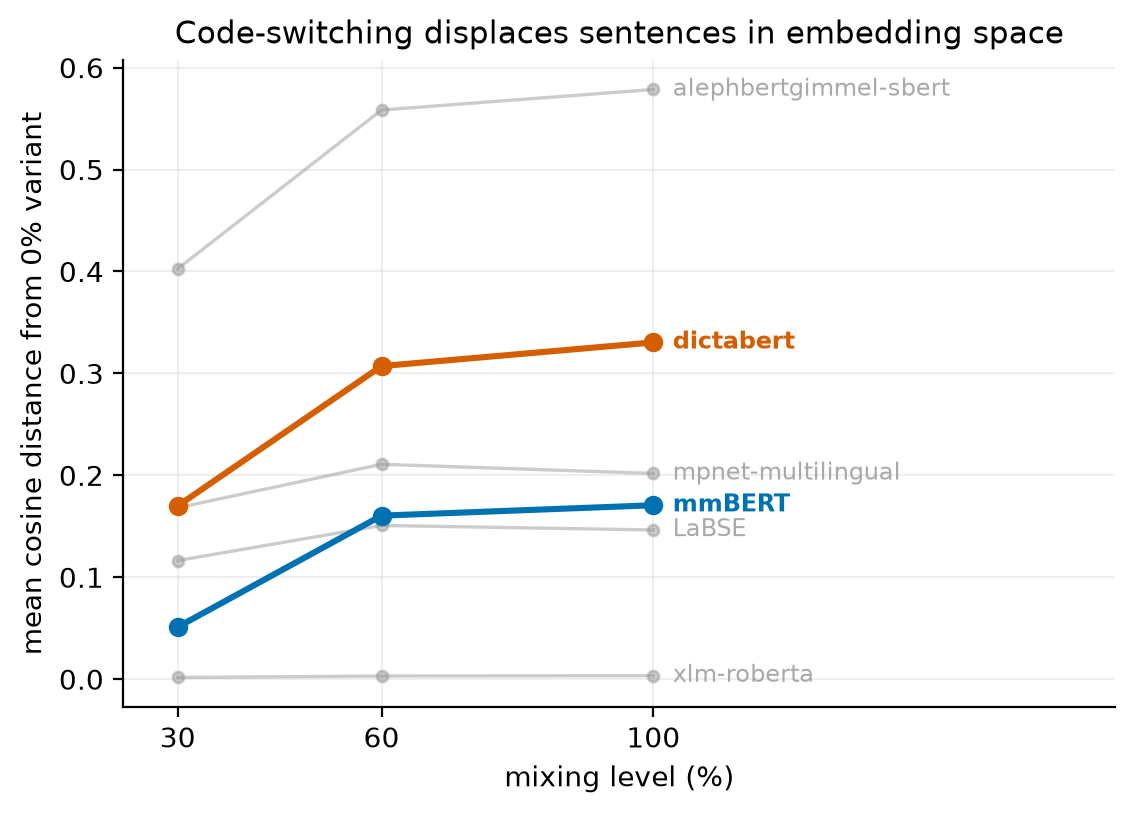
\includegraphics[width=0.82\linewidth]{fig1_embedding_drift.png}
\caption{Mean cosine distance from each seed's 0\% variant. All encoders drift
monotonically with mixing level. The Hebrew-specific DictaBERT drifts roughly
twice as far as the multilingual mmBERT.}
\label{fig:drift}
\end{figure}

Figure~\ref{fig:drift} shows that every encoder displaces sentences
monotonically as mixing increases. DictaBERT drifts about twice as far as
mmBERT ($0.330$ versus $0.171$ at 100\%). XLM-R's near-zero distances
($\approx\!0.003$) should \emph{not} be read as robustness: mean-pooled
masked-LM outputs are strongly anisotropic, compressing all cosine distances.
Its t-SNE projection separates mixing levels cleanly despite the tiny absolute
distances, so the geometry does encode mixing --- raw cosine simply cannot
resolve it for that model. Standard post-processing (mean-centering, or
whitening the embedding covariance) is known to reduce anisotropy in
masked-LM representations, but we did not apply it here; we therefore avoid
directly comparing XLM-R's absolute cosine distances with those of the other
encoders.

\subsection{Pure-Hebrew training collapses under mixing}

\begin{figure}[t]
\centering
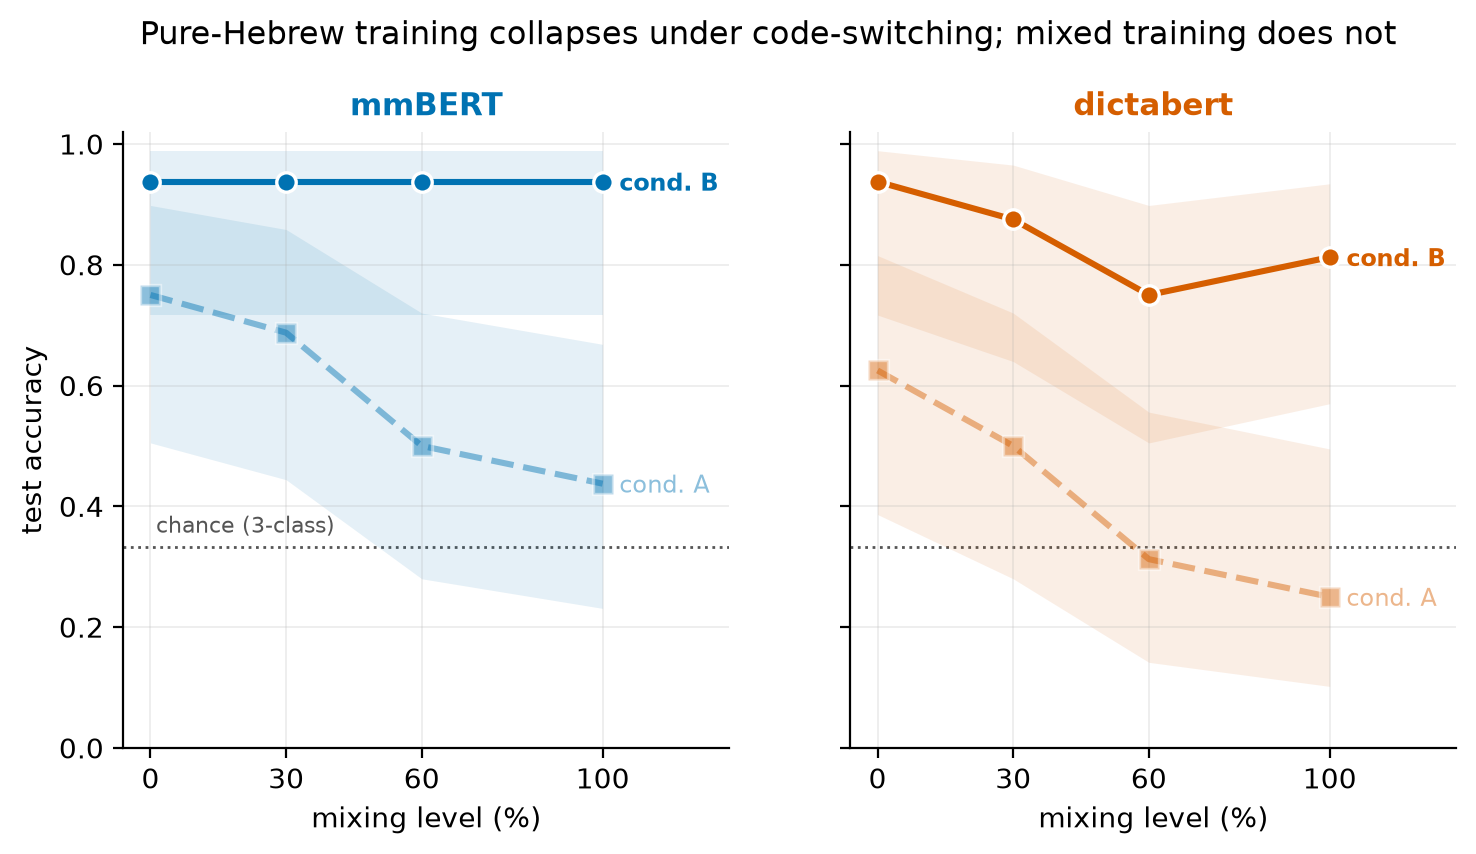
\includegraphics[width=\linewidth]{fig2_accuracy_vs_mixing.png}
\caption{Test accuracy by mixing level. Shaded bands are 95\% Wilson intervals
($n=16$ per cell). Dashed = condition A (pure-Hebrew training),
solid = condition B (mixed training). Dotted line marks 3-class chance.}
\label{fig:acc}
\end{figure}

\begin{table}[t]
\centering
\small
\begin{tabular}{llcc}
\toprule
\textbf{Model} & \textbf{Cond.} & \textbf{Pooled acc.} & \textbf{95\% CI} \\
\midrule
mmBERT    & A & 0.594 & [0.47, 0.71] \\
mmBERT    & B & \textbf{0.938} & [0.85, 0.98] \\
DictaBERT & A & 0.422 & [0.31, 0.54] \\
DictaBERT & B & 0.844 & [0.74, 0.91] \\
\bottomrule
\end{tabular}
\caption{Accuracy pooled across mixing levels ($n=64$ per condition).
Condition B beats A for both models: Fisher $p=5.4\times10^{-6}$ (mmBERT),
$p=1.1\times10^{-6}$ (DictaBERT).}
\label{tab:pooled}
\end{table}

Under condition A, both models degrade significantly as mixing rises
(Cochran--Armitage: mmBERT $z=-2.03$, $p=0.042$; DictaBERT $z=-2.34$,
$p=0.019$). The steepest fall is between 30\% and 60\% mixing --- mmBERT
$0.69\!\rightarrow\!0.50$, DictaBERT $0.50\!\rightarrow\!0.31$ --- indicating
that the transition from primarily lexical borrowing to more frequent
language alternation appears particularly challenging. At 60\% and 100\%
mixing, DictaBERT's point estimates are close to the three-class chance
level.

Condition B recovers most of the loss (Table~\ref{tab:pooled}), and we find no
statistically significant degradation across mixing level under mixed
training (mmBERT $p=1.00$, DictaBERT $p=0.24$). mmBERT
becomes completely flat at $0.938$ across all four levels. DictaBERT's
apparent dip at 60\% is \emph{not} separable from noise (CI $[0.51, 0.90]$)
and we do not interpret it.

\subsection{Specialisation appears to be a liability in this setting}

DictaBERT is worse than mmBERT at every mixing level in condition A, degrades
on a steeper trend, and remains uneven even after mixed-data training. This is
the opposite of the intuition that a Hebrew-tuned model should handle Hebrew
workplace text best: the monolingual prior is precisely what English intrusion
violates, whereas mmBERT's multilingual pretraining has already seen both
sides of the switch. With only two models compared in one synthetic
Hebrew--English setting, this should be read as evidence that specialisation
reduced robustness \emph{here}, not as a general claim about language
specialisation.

\subsection{Drift predicts accuracy loss}

\begin{figure}[t]
\centering
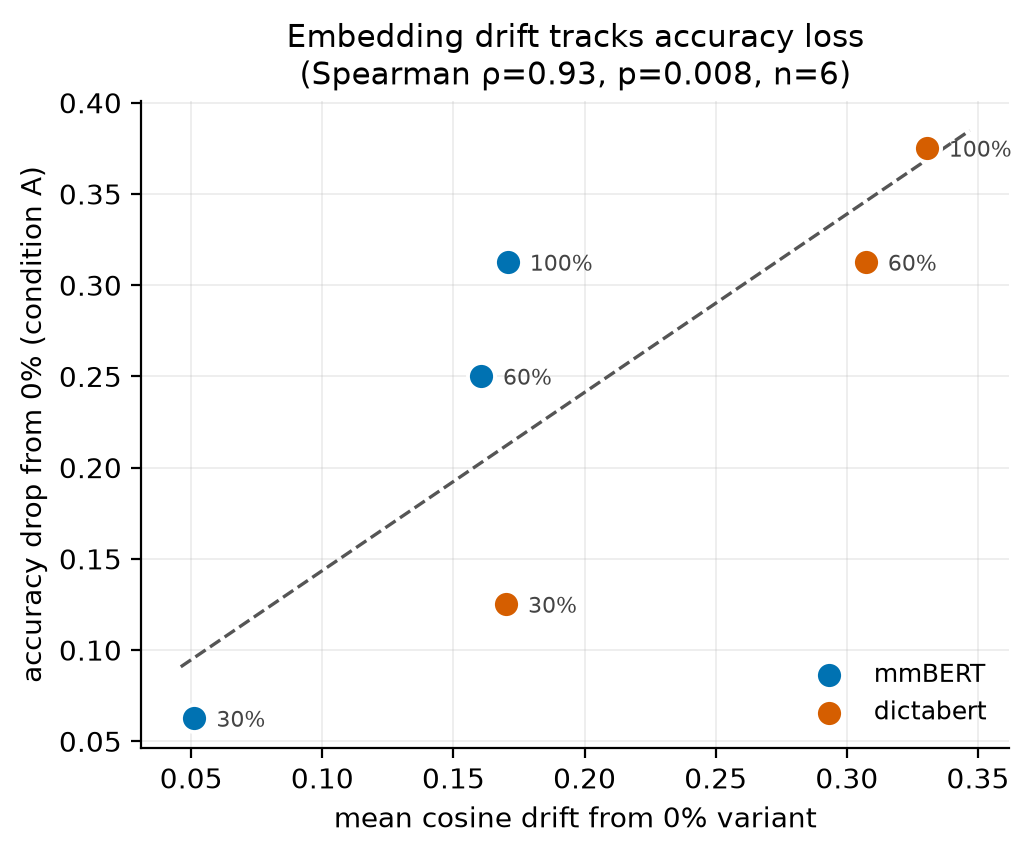
\includegraphics[width=0.75\linewidth]{fig3_drift_vs_accuracy.png}
\caption{Embedding drift versus condition-A accuracy drop from each model's
own 0\% cell. Spearman $\rho=0.93$ ($p=0.008$, $n=6$).}
\label{fig:link}
\end{figure}

Pairing each model's embedding drift against its condition-A accuracy drop
(Figure~\ref{fig:link}) gives $\rho=0.93$. With six paired points this is
descriptive rather than a powered test. It is, however, corroborated by an
observation in the same direction: the model that drifts further (DictaBERT)
is also the one that degrades further. Two complementary measurements showing
the same qualitative pattern are consistent with representational displacement
as a contributing mechanism behind the accuracy loss, though this does not
establish a causal link.

\subsection{Is this specific to sentiment?}
\label{sec:generality}

\begin{figure}[t]
\centering
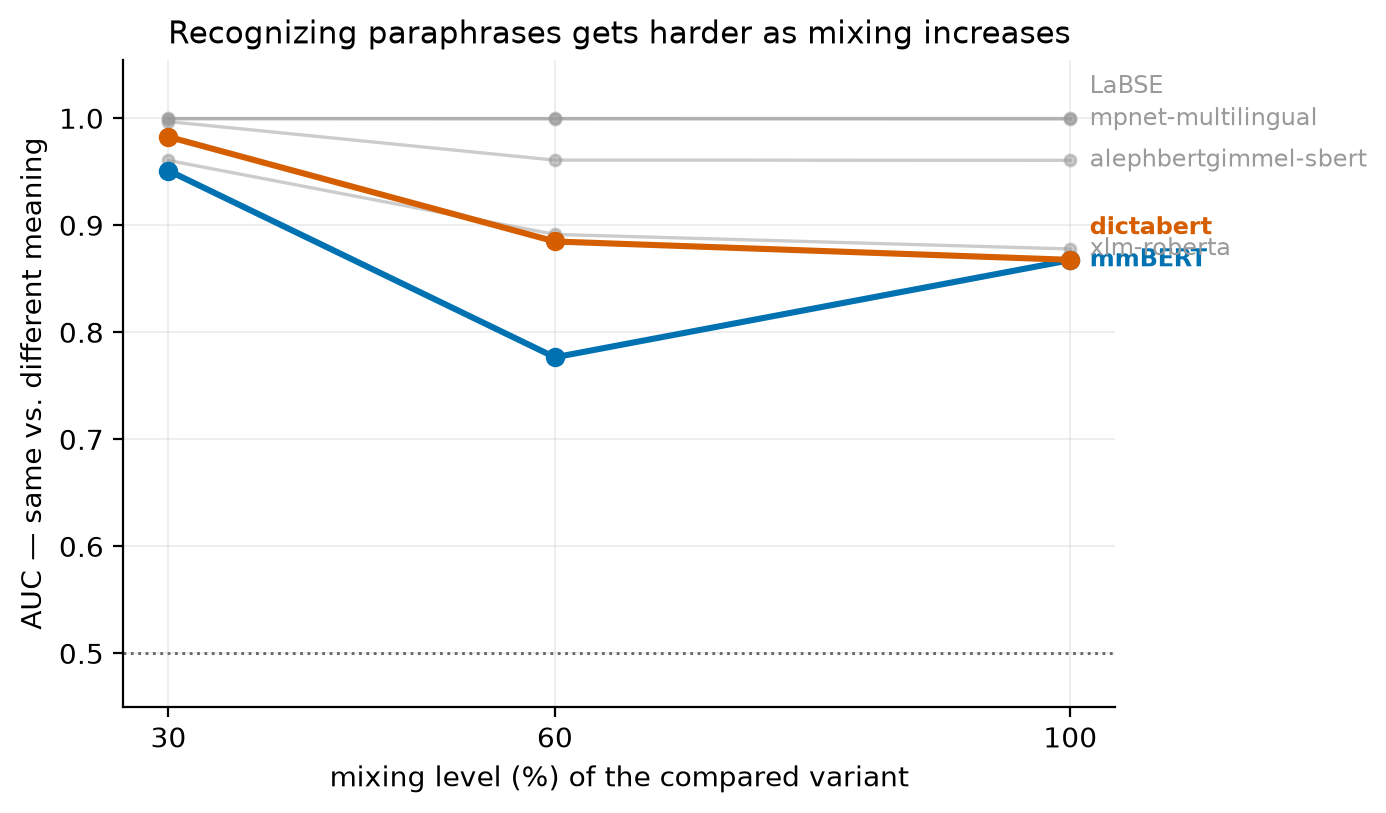
\includegraphics[width=0.75\linewidth]{fig4_semantic_equivalence.png}
\caption{AUC for distinguishing a true paraphrase (same seed, different
mixing level) from an unrelated sentence, using the embeddings from
Section~\ref{sec:results}. No new labels or training.}
\label{fig:semeq}
\end{figure}

\textbf{Semantic equivalence} (Figure~\ref{fig:semeq}) needs no labels, only
the embeddings already computed above. All six encoders separate true
paraphrases from unrelated sentences well above chance at every mixing level,
but the two fine-tuned models decline over exactly the window identified
above: mmBERT $0.95\!\rightarrow\!0.78$ and DictaBERT
$0.98\!\rightarrow\!0.89$ from 30\% to 60\% mixing. Dedicated cross-lingual
similarity models (mpnet, LaBSE) barely move, consistent with that being
closer to their training objective. This provides complementary evidence,
without depending on labeled data for a downstream task, that the observed
representational changes are not confined to the sentiment classification
setup --- though this check still relies on the same underlying embeddings
as Section~\ref{sec:drift-section}, so it is not a fully independent
replication.

\subsection{Annotator ceiling}
\label{sec:annotator-ceiling}

Both annotators (human and LLM) score 100\% at every mixing level on the
held-out test split. This is a genuine measurement but a weak ceiling: only 2
of 105 seeds drew any annotator error corpus-wide, and both fell in the
training split. It indicates that our corpus encodes sentiment unusually
unambiguously --- a property of the dataset, not evidence that the task is
easy in the wild.

\section{Discussion}

Hebrew--English code-switching measurably degrades sentiment classification,
and does so in a graded rather than binary fashion: accuracy is largely
preserved under light lexical borrowing and falls sharply once alternation
becomes structural, between 30\% and 60\% mixing. In our experimental setting,
the Hebrew-specialised encoder is the more fragile of the two --- in accuracy,
in trend steepness, and in how far its representations move --- suggesting
that specialisation to one language can become a liability when the other
intrudes. Fine-tuning on mixed data removes the measurable degradation,
reproducing on Hebrew--English what \textsc{GLUECoS} reported for Hindi- and
Spanish--English.

Extending beyond sentiment supports rather than narrows this account. A
labeling-free semantic-equivalence check degrades over the identical
30--60\% window with no labeled data involved, providing complementary
evidence that representational drift, rather than an artifact of the
sentiment classifier head, contributes to the effect.

The practical implication is direct: a Hebrew-tuned model validated on clean
Hebrew will overstate its performance on real Israeli workplace text, and a
simple and effective remedy in our setting is to place mixed-language data in
the training set. At the same time, several aspects of the setup bound how
far these results generalise: the corpus is LLM-generated rather than sampled
from real Slack messages, the test set is small (16 items per mixing-level
cell), and the 420 items come from only 105 underlying seeds, so pooled
significance tests should be read with that repeated-measures structure in
mind. The dose--response framing itself, however, is the main methodological
contribution here, and it is directly reusable for other language pairs and
other NLP tasks beyond sentiment.

\section{Code}

Code, data, and the full analysis notebook are available at:
\url{https://github.com/aviv-barel/nlp-final-project}

\bibliographystyle{plain}
\bibliography{references}

\end{document}
